\documentclass[conference]{IEEEtran}
\IEEEoverridecommandlockouts
\usepackage{cite}
\usepackage{amsmath,amssymb,amsfonts}
\usepackage{graphicx}
\usepackage{textcomp}
\usepackage{xcolor}
\usepackage{booktabs}
% Target: IEEE ICMLA (IEEE conference template, IEEEtran). Check the current CFP for page limit and anonymity.
\begin{document}
\title{K-Ont: Hyperbolic Embeddings of Ontologies and Their Knowledge-Graph Individuals, with Application to Ontology-Guided Crystal Structure Generation}
\author{
\IEEEauthorblockN{Gowtham Ramesh}\IEEEauthorblockA{Dept. of Computer Science and Engineering, Amrita Vishwa Vidyapeetham, Coimbatore, India\\ [email]} \and
\IEEEauthorblockN{Shantharam P}\IEEEauthorblockA{Dept. of Computer Science and Engineering, Amrita Vishwa Vidyapeetham, Coimbatore, India\\ [email]} \and
\IEEEauthorblockN{Sarvesha Nandhakumar}\IEEEauthorblockA{Dept. of Computer Science and Engineering, Amrita Vishwa Vidyapeetham, Coimbatore, India\\ [email]} \and
\IEEEauthorblockN{Akshay KS}\IEEEauthorblockA{Dept. of Computer Science and Engineering, Amrita Vishwa Vidyapeetham, Coimbatore, India\\ [email]} \and
\IEEEauthorblockN{RD Tarun}\IEEEauthorblockA{Dept. of Computer Science and Engineering, Amrita Vishwa Vidyapeetham, Coimbatore, India\\ [email]} \and
\IEEEauthorblockN{S Ajeth}\IEEEauthorblockA{Dept. of Computer Science and Engineering, Amrita Vishwa Vidyapeetham, Coimbatore, India\\ [email]}
}
\maketitle
\begin{abstract}
Ontology embedding models place the concepts of an ontology in a geometric space where subsumption becomes measurable, but they do not represent the individuals of a knowledge graph (KG). We present \textbf{K-Ont}, which extends the hyperbolic ontology encoder OnT to KG individuals: the materials, crystals and elements of a 5,000-material battery KG are verbalised and trained jointly with the ontology's axioms and facts in a Poincar\'e ball. On 1,018 held-out materials K-Ont types materials and crystals at 99.7--100\% and predicts battery role and structure family well above majority baselines, while matching OnT on GALEN axiom prediction; without the ontology's axioms typing falls to 64\%. A retention objective lets a single K-Ont model also retrieve crystal frameworks for unseen compositions. Used as a template retriever, it recovers the reference structure at the first attempt for 60.5\% of 902 held-out materials, versus 48.3\% for a fine-tuned CrystaLLM and 52.1\% for data-mined substitution; a plain encoder trained on the same KG relation does equally well, so the gain comes from KG retrieval, which K-Ont adds to the ontology model. Combined with CrystaLLM and a CHGNet energy check, the system commits to a single answer that is right 69.3\% vs 63.7\% of the time. On 199 novel cathode compositions, templates give CrystaLLM-large a lower-energy structure for 34 and a higher one for none, and an independent energy-above-hull calculation confirms 32 of the 34. Injecting the same knowledge into the language model, as a soft or hard prompt, adds at most 1.5 points.
\end{abstract}
\begin{IEEEkeywords}
ontology embedding, knowledge graph, hyperbolic embedding, crystal structure generation, battery materials, retrieval-augmented generation
\end{IEEEkeywords}
\section{Introduction}
Materials knowledge is increasingly curated as ontologies and knowledge graphs (KGs): battery ontologies such as BattINFO~\cite{clark2022battinfo} fix a vocabulary of materials, structures and electrode roles, and pipelines populate KGs with facts drawn from databases such as the Materials Project~\cite{jain2013mp}. Generative models for crystals~\cite{xie2022cdvae,jiao2023diffcsp,antunes2024crystallm,zeni2025mattergen}, on the other hand, learn from structure files alone and do not use this curated knowledge.

Ontology embeddings offer a bridge. Hyperbolic models embed hierarchies with low distortion~\cite{nickel2017poincare}; language-model encoders such as HiT~\cite{he2024hit} and OnT~\cite{yang2025ont} embed the \emph{names} of ontology concepts in a Poincar\'e ball so that subsumption and existential restrictions become geometric. These encoders, however, represent concepts (the TBox) only; the individuals of a KG (the ABox) --- the actual materials and crystals one wants to reason about and generate --- are not embedded.

This paper makes four contributions:

\begin{itemize}
\item \textbf{K-Ont}, an extension of OnT to KG individuals: individuals are verbalised and trained jointly with the ontology's axioms, typing facts and relation facts in one hyperbolic space (Sec. III).
\item An evaluation on a 5,000-material battery KG with held-out materials, on OnT's GALEN benchmark, and on a second (medical) domain, including an ontology ablation and a retention objective that lets \textbf{one} K-Ont model hold the original ontology, a new domain ontology and KG, and a crystal-retrieval skill (Sec. V-A, V-B).
\item \textbf{K-Ont-guided template generation}: K-Ont retrieves known crystal frameworks for a target composition, which are built directly by element substitution; at the first attempt it outperforms a fine-tuned crystal language model and the standard data-mined substitution method, and complements the language model on novel cathodes (Sec. V-C, V-E).
\item A controlled negative result: injecting the same knowledge \emph{into} a crystal language model, as a soft prompt or as a retrieved hard prompt, yields at most a small gain, and we measure why (Sec. V-D).
\end{itemize}
\section{Related Work}
\textbf{Ontology and KG embeddings.} Translational KG embeddings~\cite{bordes2013transe} model relations between entities but not the logical structure of an ontology. Poincar\'e embeddings~\cite{nickel2017poincare} showed that hyperbolic space suits hierarchies; HiT~\cite{he2024hit} re-trains a sentence encoder~\cite{reimers2019sbert,wang2020minilm} so that its outputs live in a Poincar\'e ball and encode subsumption, and OnT~\cite{yang2025ont} extends this to EL ontologies with role rotations for existential restrictions, evaluated on several real-world ontologies including GALEN, GO and ANATOMY. Geometric EL embeddings~\cite{kulmanov2019elem,jackermeier2024box2el} and OWL2Vec$^*$~\cite{chen2021owl2vec} also handle individuals, but as graph nodes or symbols rather than through a language model over their descriptions, so an unseen individual cannot be embedded from its text. Ontology preprocessing commonly relies on DeepOnto~\cite{he2024deeponto}. The language-model encoders HiT and OnT embed concepts only; embedding KG individuals in the same model is the gap K-Ont addresses.

\textbf{Crystal structure generation.} Diffusion and variational models~\cite{xie2022cdvae,jiao2023diffcsp,zeni2025mattergen} and autoregressive language models over CIF text~\cite{antunes2024crystallm} generate structures from compositions or properties. Substitution-based prediction reuses known prototypes; Hautier et al.~\cite{hautier2011} learn ion-substitution probabilities from data and remain a strong, widely used baseline. Retrieval-augmented generation~\cite{lewis2020rag} and prompt or prefix tuning~\cite{lester2021prompt,li2021prefix} are the two standard ways to condition a language model on external knowledge; we test both.

\section{Method}
\begin{figure*}[t]
\centering
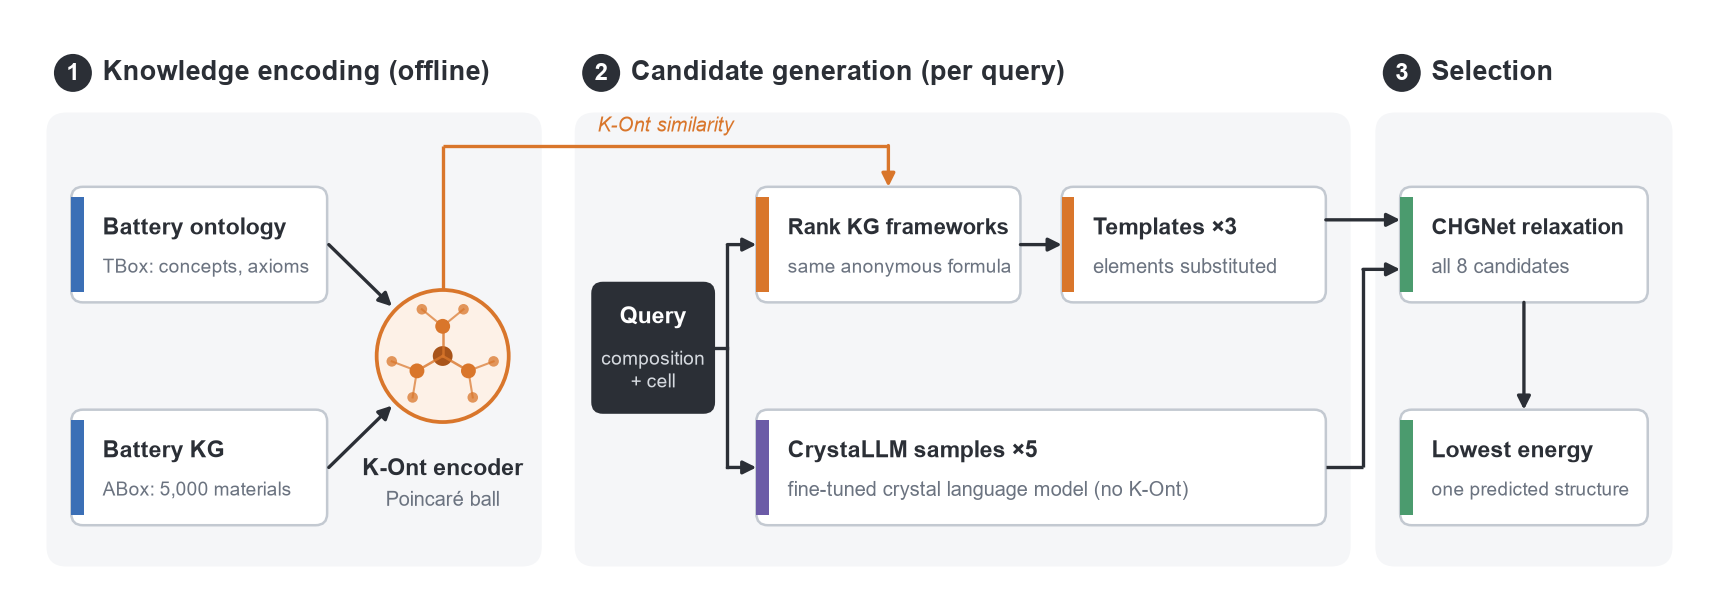
\includegraphics[width=\textwidth]{figs/overview.png}
\caption{Overview. K-Ont embeds the battery ontology and the KG's individuals in one hyperbolic space; for a new composition it ranks KG frameworks, whose sites receive the target's elements (templates); templates and language-model samples are relaxed with CHGNet and the lowest-energy structure is the answer.}
\label{fig:overview}
\end{figure*}
Fig.~\ref{fig:overview} summarises the approach: a battery KG and its ontology are embedded by K-Ont (Sec. III-B, III-C), which then guides crystal structure generation by retrieving templates (Sec. III-D).

\subsection{Battery knowledge graph}
The KG was built with the battGPT pipeline from Materials Project data~\cite{jain2013mp} and pymatgen analysis~\cite{ong2013pymatgen}: 5,000 Li/Na materials ($\le$0.15 eV/atom above hull, $\le$40 sites, 2--5 elements, 527 polymorph groups), 5.6 M triples, linked to a battery ontology with structure families (e.g. olivine, NASICON, layered oxide) and electrode roles. Each material has a crystal, its elements, properties (band gap, formation energy, hull distance, moduli, magnetisation), and relations \emph{has structure}, \emph{has structure family} and \emph{belongs to electrode}. Structure-family and role labels are assigned by rules over composition and space group.

\subsection{K-Ont}
OnT maps the name $x$ of a concept to a point $f(x)$ in a Poincar\'e ball $\mathbb{B}_c$ and scores a subsumption $C \sqsubseteq D$ with

\begin{equation}s(C,D) = -\big(d_c(f(C),f(D)) + \lambda\,(\lVert f(D)\rVert_c - \lVert f(C)\rVert_c)\big),\end{equation}
where $d_c$ is the hyperbolic distance and $\lVert\cdot\rVert_c$ the distance to the origin; an existential restriction $\exists r.D$ is embedded by a learned rotation of $f(D)$ conditioned on the role $r$~\cite{yang2025ont}. \textbf{K-Ont} keeps this model and objective and adds the ABox: each individual is verbalised as a short multi-line sentence (name, formula, chemical system, properties, space group, lattice, sites; label lines omitted), and three kinds of training rows are merged --- the ontology's TBox axioms (oversampled to 15\% of type rows and 5\% of relation rows), ABox typing rows (individual $\sqsubseteq$ class, e.g. a material $\sqsubseteq$ \emph{substance}) and ABox relation rows (material $\sqsubseteq \exists$\emph{has structure}.crystal). For relation rows we add an in-batch contrastive term so that an individual must prefer its own filler over another row's. Training starts from OnT-MiniLM-L12-galen (384-d), batch 32, 3 epochs.

\subsection{Framework relation and retention}
To retrieve crystal templates, K-Ont is taught one more KG relation, \emph{has the framework of}: for a training material, its structure-free sentence (no space group, lattice or volume; only what is known for a new composition) should score highest against pool materials of the same anonymous formula and space group, with candidates of the same formula type as negatives (listwise softmax). Learning this alone erases K-Ont's typing (catastrophic forgetting~\cite{kirkpatrick2017ewc}), so we add a \textbf{retention} term: the mean-squared distance between the current and the original embeddings of (i) all 10,108 KG sentences, (ii) 20,000 GALEN concept names held at the original OnT-galen embeddings, and (iii) the 23 relation names and role/family label phrases that drive the role rotations, each as its own term in every step. We call the resulting single model K-Ont-52c.

\subsection{Template generation and selection}
For a target composition, candidates are KG materials with the same anonymous formula and a different formula. A gradient-boosted ranker combines candidate popularity and cell size, the KG's property facts, and the K-Ont retrieval score (out-of-fold). The target's elements are placed on the top-$k$ candidates' sites (element order by amount, then electronegativity; lattice scaled by atomic radii) --- a template. For a single answer, templates and language-model samples are relaxed briefly with CHGNet~\cite{deng2023chgnet} and the lowest energy per atom wins.

\subsection{Injection baselines}
For comparison we condition CrystaLLM-small~\cite{antunes2024crystallm} on the same knowledge: (a) a \textbf{soft prompt} --- the K-Ont embedding of the retrieved template's framework as 8 prefix tokens plus gated per-layer adapters~\cite{li2021prefix}, trained with 6,453 counterfactual structures (a training composition placed in a different framework) so that the vector must be read; and (b) a \textbf{hard prompt} --- the retrieved template's CIF header (space group, cell, volume, $Z$) as the prompt, from which the model writes the atom sites~\cite{lewis2020rag}.

\section{Experimental Setup}
K-Ont is trained on 3,982 KG materials and evaluated on 1,018 held-out materials (polymorph groups kept on one side). All crystal experiments use the 902 held-out materials that have at least one same-formula-type candidate; candidates, retrievers, rankers and generators see only K-Ont's training materials. A material's structure is \emph{recovered} when a candidate matches the reference under pymatgen's StructureMatcher (length tol. 0.2, site tol. 0.3, angle 5$^\circ$); we report found@$k$. Novel compositions (200 cathode substitution children not in Materials Project, charge-balanced with SMACT~\cite{davies2019smact}) are compared by the lowest CHGNet energy after relaxation. Differences are paired over materials with 95\% bootstrap intervals~\cite{efron1994bootstrap}; pass criteria for the injection experiments were fixed before the runs. All models were trained and evaluated on one laptop GPU (RTX 4060, 8 GB).

\section{Results}
\subsection{K-Ont learns the ontology and the KG}
\begin{table}[t]
\centering
\caption{K-Ont on 1,018 held-out materials (H@1; MRR for the hierarchy). Role/family: label lines removed from the sentence; majority-class baselines 84\% / 47\%.}
\label{tab:checks}
\footnotesize
\setlength{\tabcolsep}{3pt}
\begin{tabular}{lccccc}
\toprule
Model & Mat. typing & Cryst. typing & Role & Family & TBox MRR \\
\midrule
OnT-galen (untrained on KG) & 0.000 & \textbf{1.000} & 0.67 & 0.30 & 0.28 \\
\textbf{K-Ont} & \textbf{1.000} & 0.997 & \textbf{1.000} & \textbf{0.988} & \textbf{0.969} \\
K-Ont without TBox axioms & 0.641 & 0.639 & \textbf{1.000} & 0.977 & 0.313 \\
K-Ont-52c (one model, 3 seeds) & 0.92--0.95 & \textbf{1.000} & 0.99--1.00 & \textbf{0.988} & \textbf{0.969} \\
\bottomrule
\end{tabular}
\end{table}
K-Ont generalises its typing and both ontology relations to unseen materials (Table~\ref{tab:checks}). Removing the ontology's TBox axioms (keeping all KG facts) drops material and crystal typing to 64\% and the hierarchy MRR from 0.97 to 0.31, while roles and families, which come from relation facts, survive: the ontology is what gives K-Ont its type reasoning. Because the KG's role and family labels are rule-based, near-perfect scores partly reflect learning those rules. On a second domain (303 patients of the UCI heart-disease data~\cite{detrano1989heart} verbalised as KG individuals), K-Ont patient embeddings outperformed OnT's by +2.2 AUC on average over five classifiers (four significant) and by +4.3 when three columns were missing.

\begin{figure*}[t]
\centering
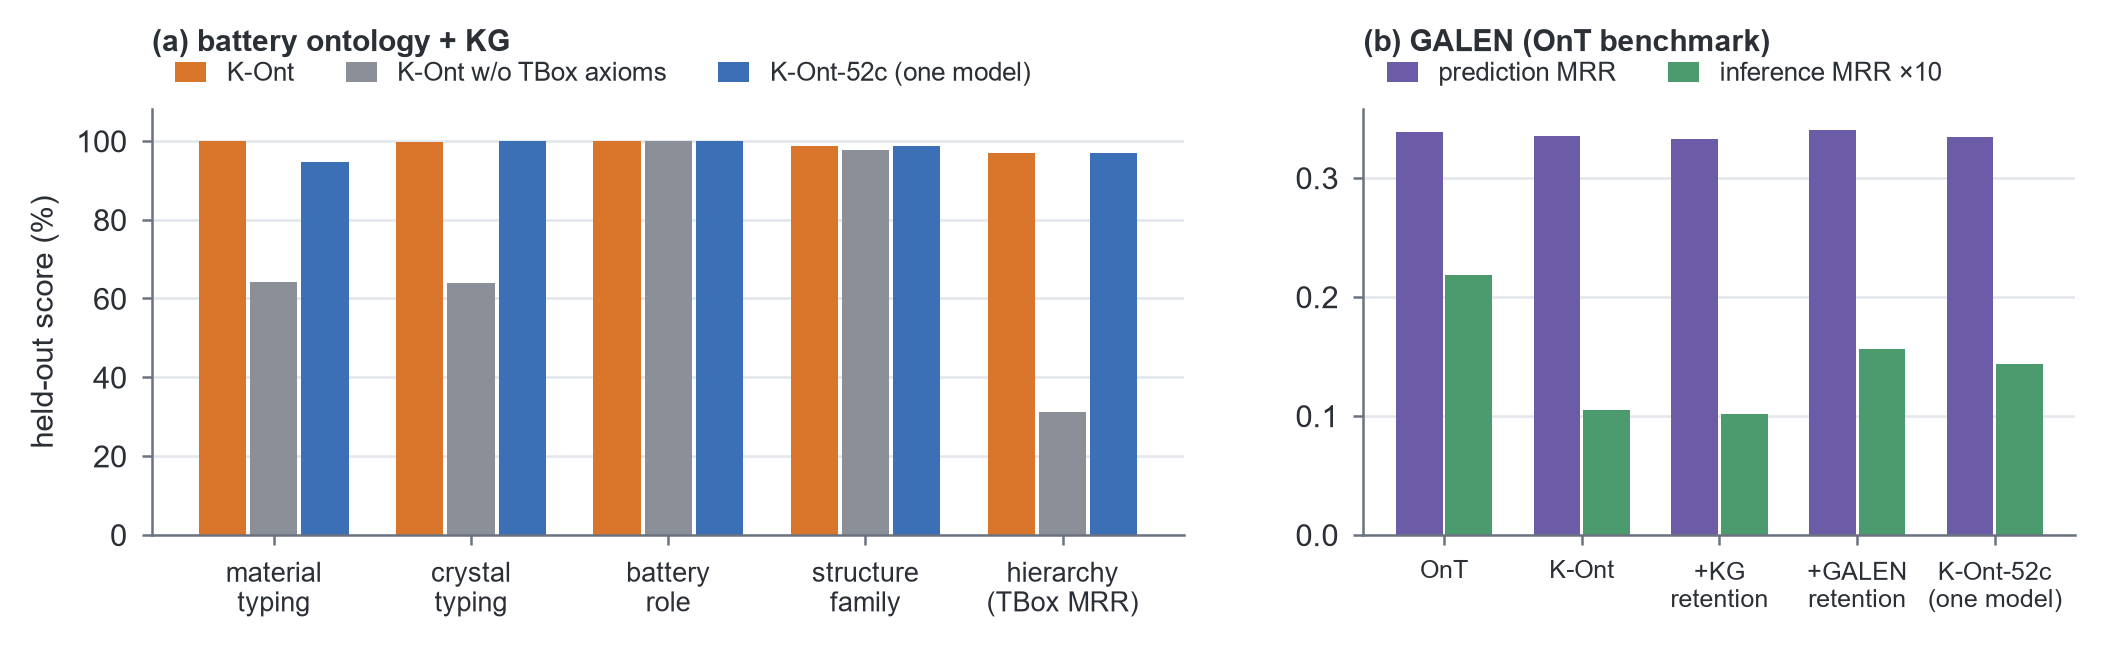
\includegraphics[width=\textwidth]{figs/kont_checks.png}
\caption{(a) K-Ont on held-out materials, without the ontology's TBox axioms, and the one-model K-Ont-52c. (b) GALEN mean reciprocal rank for OnT and K-Ont variants (inference MRR scaled $\times$10).}
\label{fig:checks}
\end{figure*}
Fig.~\ref{fig:checks}(a) shows the same comparison graphically: removing the axioms hits typing and the hierarchy, not roles and families.

\subsection{One model for GALEN, the battery KG and crystal retrieval}
\begin{table}[t]
\centering
\caption{GALEN (OnT benchmark) and crystal retrieval. Pred./inf. = prediction / inference test sets, MRR and AUC; retrieval = template found@1 on 902 held-out materials.}
\label{tab:galen}
\footnotesize
\setlength{\tabcolsep}{3pt}
\begin{tabular}{lccc}
\toprule
Model & Pred. MRR / AUC & Inf. MRR / AUC & Retr. @1 \\
\midrule
OnT-galen~\cite{yang2025ont} & 0.339 / \textbf{0.978} & \textbf{0.022 / 0.973} & -- \\
K-Ont & 0.335 / 0.952 & 0.011 / 0.918 & -- \\
+ framework, KG retention & 0.333 / 0.955 & 0.010 / 0.934 & 55.0 \\
+ GALEN retention & \textbf{0.341} / 0.976 & 0.016 / 0.961 & \textbf{55.5}$^\dagger$ \\
\textbf{K-Ont-52c} (+ anchors) & 0.334--0.339 / 0.975 & 0.014 / 0.95 & 54.2--54.8 \\
native relation, hard neg. & 0.324 / 0.960 & 0.008 / 0.896 & 54.4$^\ddagger$ \\
\bottomrule
\end{tabular}
\end{table}
Learning the battery KG costs part of OnT's GALEN inference ranking (Table~\ref{tab:galen}). Retaining KG sentences alone keeps the battery checks; adding GALEN concepts restores GALEN but ($\dagger$) collapses the role/family checks (0.025 / 0.000) until the relation phrases are retained as well. K-Ont-52c keeps every battery check of Table~\ref{tab:checks}, matches OnT on GALEN prediction, recovers about a quarter of the inference loss, and retrieves frameworks, on three seeds. Training the relation natively inside K-Ont's objective with hard negatives ($\ddagger$) matches the retrieval but collapses typing (0.09 / 0.001), so a separate fine-tune with retention is the better recipe.

\subsection{Template generation versus language-model generation}
\begin{figure}[t]
\centering
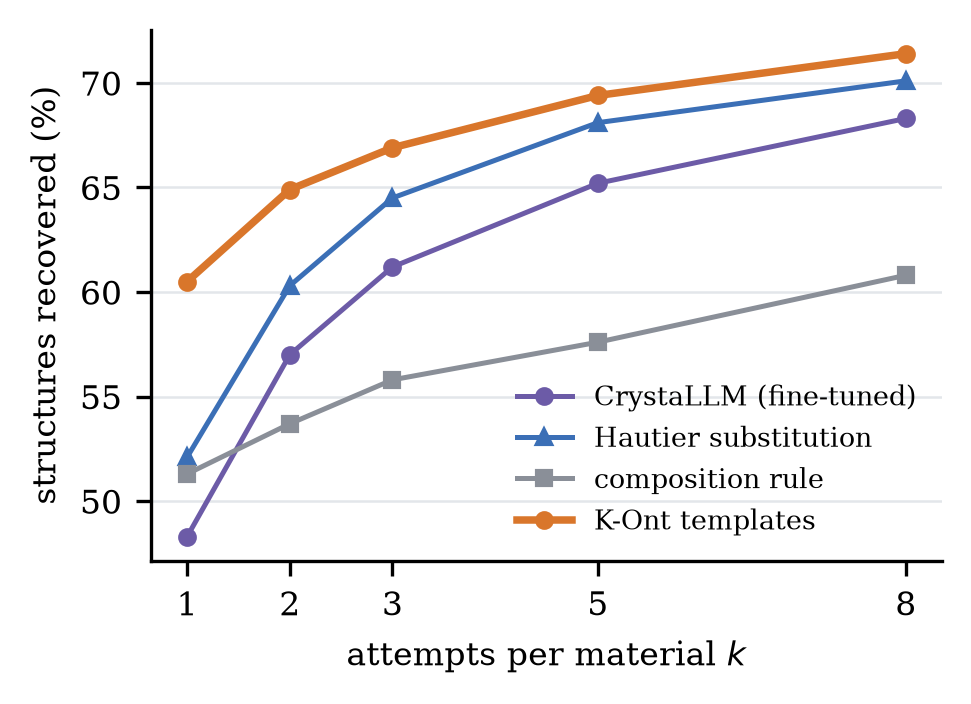
\includegraphics[width=\columnwidth]{figs/foundk.png}
\caption{Structures recovered within $k$ attempts on 902 held-out materials: K-Ont-guided templates vs a fine-tuned CrystaLLM, Hautier substitution and a composition rule.}
\label{fig:foundk}
\end{figure}
\begin{table}[t]
\centering
\caption{Found@k (\%) on 902 held-out materials, and single-answer accuracy (CHGNet lowest energy among 8 candidates, random 300 materials).}
\label{tab:found}
\footnotesize
\setlength{\tabcolsep}{3pt}
\begin{tabular}{lccc}
\toprule
Method & @1 & @3 & @8 \\
\midrule
CrystaLLM, fine-tuned~\cite{antunes2024crystallm} & 48.3 & 61.2 & 68.3 \\
Template, composition rule & 51.3 & 55.8 & 60.8 \\
Template, Hautier~\cite{hautier2011} & 52.1 & 64.5 & 70.1 \\
Template, KG ranker w/o K-Ont & 56.3 & 63.2 & 68.4 \\
\textbf{Template, K-Ont ranker} & \textbf{60.5} & 66.9 & 71.4 \\
Template, plain-encoder ranker & \textbf{60.5} & 67.6 & 72.7 \\
3 templates + 5 CrystaLLM & -- & -- & \textbf{77.3} \\
Single answer: CrystaLLM, 8 samples & 63.7 &  &  \\
Single answer: 3 templ. + 5 CrystaLLM & \textbf{69.3} &  &  \\
\bottomrule
\end{tabular}
\end{table}
K-Ont-guided templates recover the reference structure at the first attempt +12.2 points [9.0, 15.4] more often than the fine-tuned CrystaLLM, +8.4 [5.5, 11.2] more than Hautier substitution and +9.2 more than the composition rule (Fig.~\ref{fig:foundk}, Table~\ref{tab:found}); CHGNet relaxation of the templates changes this by +0.3. From five attempts Hautier substitution comes within about 1.3 points. The two generators get different materials right: three templates plus five CrystaLLM samples reach 77.3\% versus 68.3\% for eight samples [+6.9, +11.1]. When one answer must be chosen by CHGNet energy, the combined pool is right 69.3\% versus 63.7\% for CrystaLLM choosing among its own eight samples (+5.7 [1.3, 9.7]); with this physics selection the template alone (61.7\%) no longer beats CrystaLLM. For template choice itself, a plain encoder fine-tuned on the same KG relation is as good as K-Ont (60.5 vs 60.5 at $k=1$); K-Ont's starting weights help only with 5\% of the training data (+3.4 on the space group; Fig.~\ref{fig:lc}). The distinct value of K-Ont is doing this within the same model as the ontology reasoning.

\begin{figure*}[t]
\centering
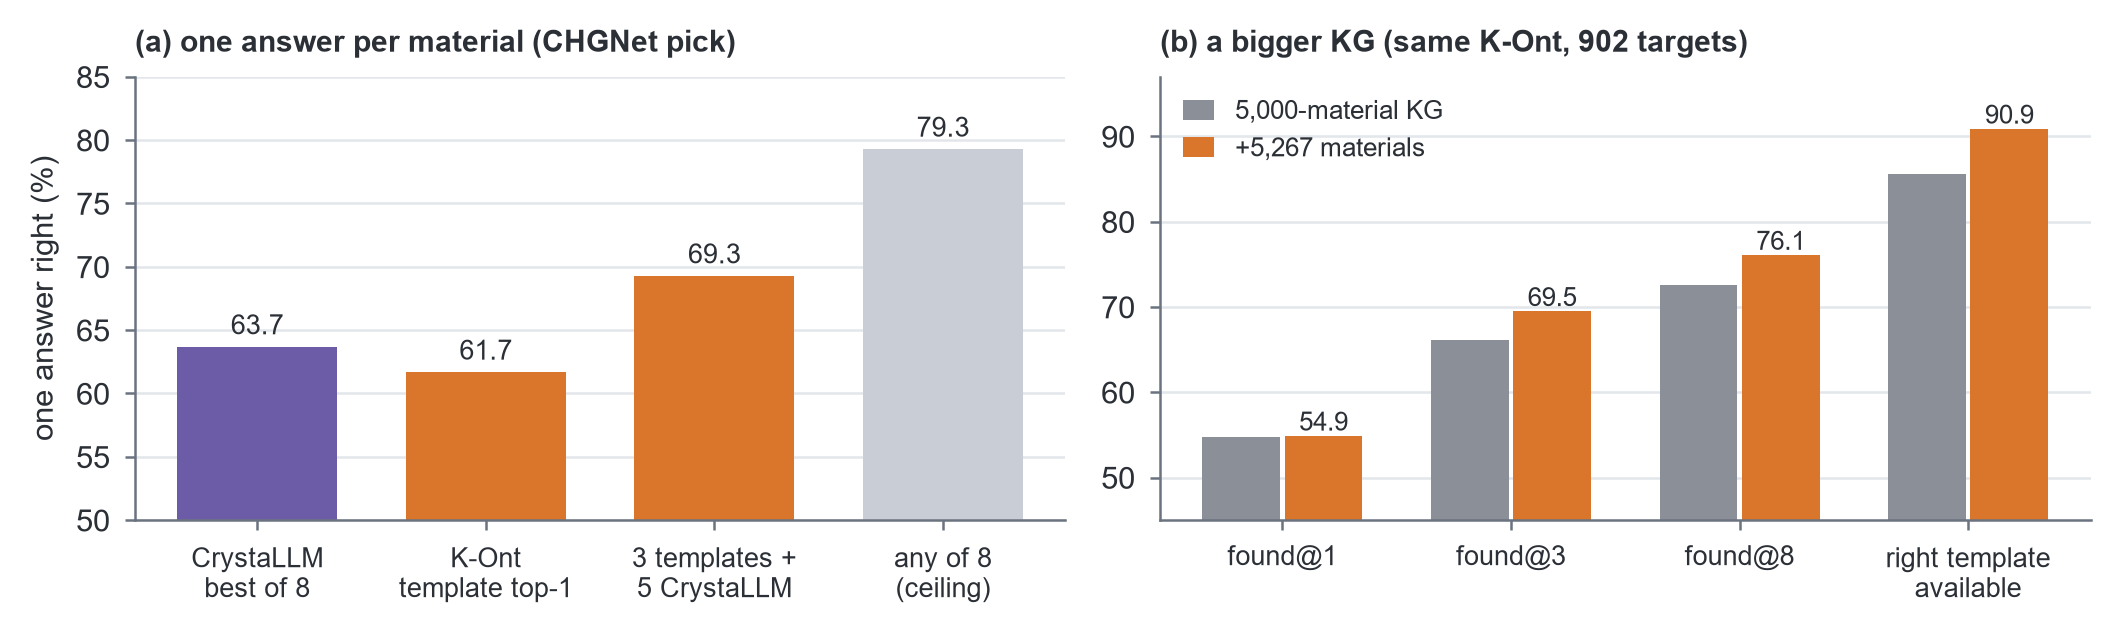
\includegraphics[width=\textwidth]{figs/system.png}
\caption{(a) One committed answer per material (CHGNet lowest energy among 8 candidates, random 300 of the 902 targets). (b) The same K-Ont-52c retriever with the 5,000-material KG and with 5,267 further KG materials: structures found within k attempts, and targets for which some candidate has the true space group.}
\label{fig:system}
\end{figure*}
\begin{figure}[t]
\centering
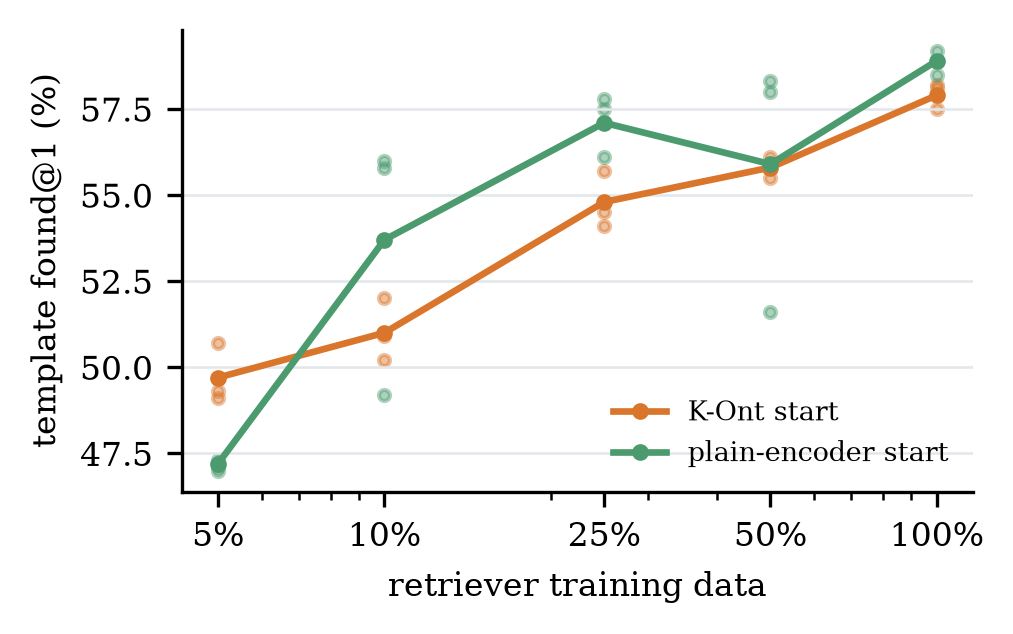
\includegraphics[width=\columnwidth]{figs/learning_curve.png}
\caption{Retriever learning curve: template found@1 when the retriever is fine-tuned from K-Ont or from the plain encoder on 5--100\% of the KG examples (lines: mean, dots: 3 seeds).}
\label{fig:lc}
\end{figure}
Fig.~\ref{fig:system}(a) summarises the single-answer system and Fig.~\ref{fig:system}(b) the effect of a larger KG: extending the pool with 5,267 further materials raises the share of targets with a correct candidate from 85.6\% to 90.9\% and found@3 / found@8 by +3.4 [1.7, 5.2] / +3.4 [1.9, 5.1], without retraining K-Ont; the first pick does not change.

\subsection{Injecting K-Ont knowledge into the language model}
\begin{table}[t]
\centering
\caption{True-structure share (\%) of generated samples, 902 held-out materials $\times$ 8 samples. Ceiling: the analogue with the true framework.}
\label{tab:inj}
\footnotesize
\setlength{\tabcolsep}{3pt}
\begin{tabular}{lcc}
\toprule
Arm & CrystaLLM & From-scratch GPT \\
\midrule
Plain fine-tune (no K-Ont) & \textbf{47.5} & 20.6 \\
Soft prompt, K-Ont-ranked analogue & 44.1 & \textbf{22.1} \\
Soft prompt, random analogue & 22.7 & 11.1 \\
Soft prompt, true analogue (ceiling) & 49.6 & 23.3 \\
Hard prompt (template CIF header) & 45.9$^*$ & -- \\
\bottomrule
\end{tabular}
\end{table}
A K-Ont soft prompt clearly steers the generated framework (random vs retrieved analogue: -21.4 points), but on CrystaLLM it never beats plain fine-tuning, and even the true analogue adds only +2.1: CrystaLLM was pre-trained on Materials Project and recalls these structures (Table~\ref{tab:inj}). We therefore pre-trained a 25 M-parameter GPT with CrystaLLM's architecture from scratch on 300,000 CrystaLLM training structures with every evaluation composition removed. Without memorisation the soft prompt helps (+1.5 [0.5, 2.5]), but the ceiling stays at +2.7: the vector identifies the framework while the model still writes every coordinate. A hard prompt with the retrieved template's header ($^*$found@1) is worse than using the template itself (60.5\%). Knowledge is most useful outside the generator (Fig.~\ref{fig:inj}).

\begin{figure}[t]
\centering
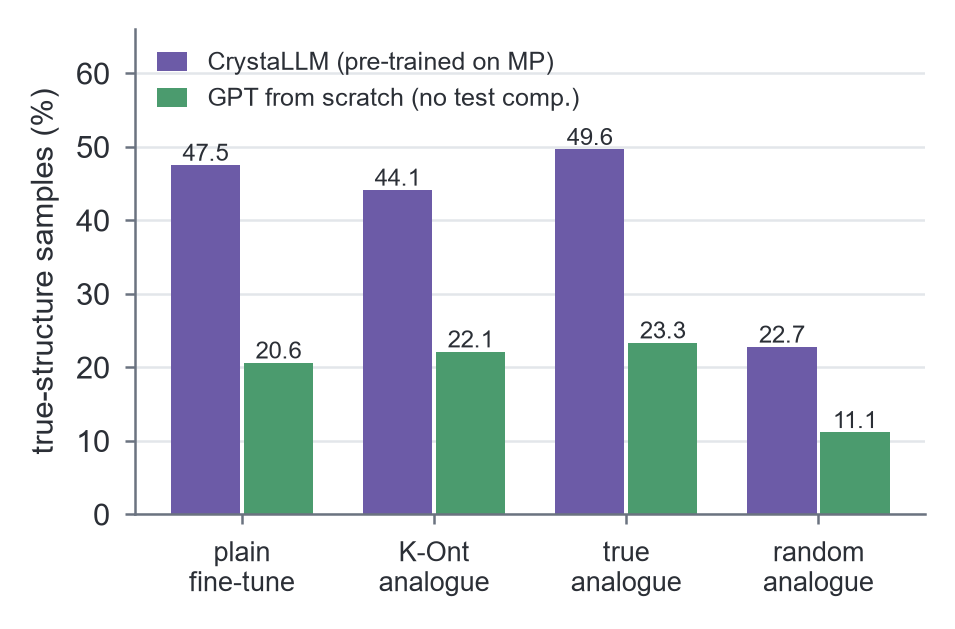
\includegraphics[width=\columnwidth]{figs/injection.png}
\caption{Injecting K-Ont knowledge as a soft prompt: true-structure share of generated samples for a model that has seen Materials Project (CrystaLLM) and one pre-trained from scratch without the evaluation compositions.}
\label{fig:inj}
\end{figure}
\subsection{Novel cathode compositions}
\begin{table}[t]
\centering
\caption{Novel cathodes (not in Materials Project). Top: lowest CHGNet energy per composition vs CrystaLLM-large's best of 10 (199 compositions, 5 meV/atom tie band). Bottom: independent energy-above-hull check of the 34 compositions where the template was lower.}
\label{tab:novel}
\footnotesize
\setlength{\tabcolsep}{3pt}
\begin{tabular}{lccc}
\toprule
 & Lower & Tie & Higher \\
\midrule
3 K-Ont templates & 34 & 126 & 39 \\
K-Ont templates + CrystaLLM-large & \textbf{34} & 165 & \textbf{0} \\
Independent $E_{hull}$, K-Ont template & \textbf{32} & 1 & 1 \\
\bottomrule
\end{tabular}
\end{table}
On compositions with no reference structure, three K-Ont templates are statistically level with CrystaLLM-large's best of ten (+1.3 meV/atom [-4.1, 6.4]); adding them to CrystaLLM finds a lower-energy structure for 34 of 199 compositions and a higher one for none (-7.5 meV/atom [-11.8, -4.0]) (Table~\ref{tab:novel}). An independent energy-above-hull calculation [TODO: method, e.g. DFT functional and settings] of those 34 places the template lower in 32; median 0.025 vs 0.088 eV/atom, with 23 vs 13 within 50 meV/atom of the hull (Fig.~\ref{fig:ehull}). These 34 were selected by CHGNet, so this confirms the ranking rather than an unbiased rate.

\begin{figure}[t]
\centering
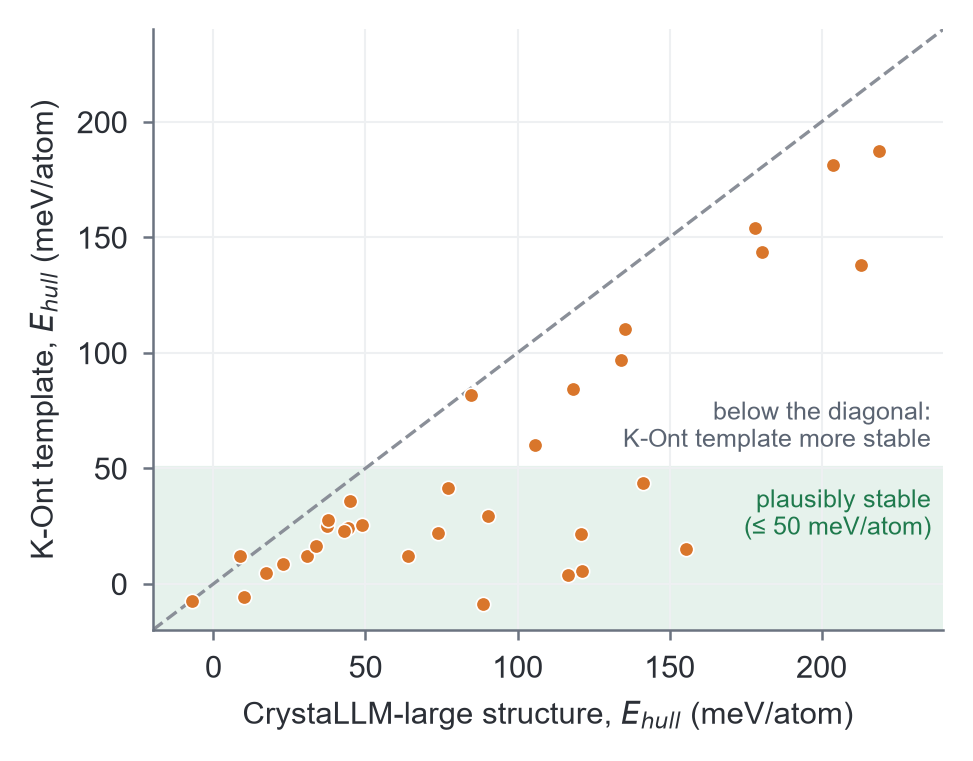
\includegraphics[width=\columnwidth]{figs/novel_ehull.png}
\caption{Independent energy above hull of the K-Ont template vs the CrystaLLM-large structure for the same novel composition (33 of 34; LiCo$_2$BiO$_4$, about 4 eV/atom for both, omitted). Points below the diagonal: the template is more stable.}
\label{fig:ehull}
\end{figure}
\section{Discussion and Limitations}
\begin{itemize}
\item \textbf{Rule-based labels.} The KG's roles and families are rule-assigned; very high scores partly reflect the rules.
\item \textbf{K-Ont versus a plain encoder.} For template choice alone, a plain encoder trained on the same KG relation is as good; K-Ont's contribution is a single model that also reasons over the ontology (whose axioms the ablation shows are necessary) and keeps the original ontology.
\item \textbf{Memorisation.} Known-material benchmarks favour generators pre-trained on the same database; the from-scratch control and the novel-composition test address this, the latter only energetically (no synthesis or electrochemical validation).
\item \textbf{Template coverage.} Templates cannot produce frameworks absent from the KG; a larger KG raises coverage and found@3/@8 without retraining (Fig.~\ref{fig:system}b) but not the first pick, and about 9\% of targets still have no correct candidate.
\item \textbf{Scope.} One crystal KG; costs of the one-model recipe are material typing (0.92--0.95) and part of GALEN inference.
\end{itemize}
\section{Conclusion}
K-Ont extends hyperbolic ontology embeddings from concepts to knowledge-graph individuals. It learns a battery ontology and KG, keeps its original ontology, and --- with a retention objective covering KG sentences, original concepts and relation phrases --- holds a crystal-retrieval skill in the same model. As a template retriever it outperforms a fine-tuned crystal language model and data-mined substitution at the first attempt, and it complements the language model on novel cathodes, whereas injecting the same knowledge into the language model helps little. Future work: larger and expert-curated KGs, DFT validation at scale, and generators that edit retrieved templates rather than write structures from scratch.

\bibliographystyle{IEEEtran}
\bibliography{refs}
\end{document}